%!TEX root = ../thesis.tex

\chapter{Background - Tools and Technologies}
\label{ch:background}

\section{Blockchain}
Blockchain \cite{p2p-bitcoin} serves as a ledger between untrusting parties. All the untrusting parties start participating in the peer-to-peer (p2p) network as peers and the algorithm allows for direct transactions to take place between the participating parties. Eliminating the need for a central authority maintaining the transactions altogether. All the transactions are vetted to be valid and non-malicious before being added to a block and becoming a permanent part of the chain. Once a block has been admitted into the chain, it can never be removed from the ledger. 

\bigskip
The validation of whether to add a block to the chain is done through a consensus algorithm. There is a choice of consensus algorithms dictating how a transaction is accepted into the chain. Over time several consensus algorithms have been developed each with its pros and cons. Normally it is a trade-off between speed and security, but the algorithms are being improved upon to come up with a consensus algorithm that is both fast and safe. Bitcoin uses an algorithm called proof-of-work as a consensus, which ensures the miner has done enough amount of work to add the block to the chain and that to change it the same amount of work would go into mining every subsequent block. It has its shortcomings. Proof of Work is slow and energy inefficient, Ethereum is proposing to move to a proof-of-stake algorithm for consensus, where the network holds on to the stake of the miner till it is verified that the blocks added are valid. The takeaway point here is that the consensus algorithm is one of the core things setting apart a blockchain from other blockchain networks. As we will discuss later, Hyperledger uses a consensus algorithm where the transactions have to be signed by the peers according to a policy before being added to the chain, the benefit of having a private chain with identified entities.

\bigskip
The distributed ledger technology is a lot older than Bitcoin. \cite{blind-signatures} and \cite{secure-names} are papers from the 90's discussing the establishment of a distributed ledger in a peer-to-peer network. Bitcoin was the practical implementation of the algorithm as a crypto-currency in 2008 by researcher(s) under the assumed name of Satoshi Nakamoto. As discussed earlier, Bitcoin uses something known as proof-of-work as the consensus algorithm where each transaction is timestamped and its hash included in the chain ensuring that changing a transaction demands all the transactions afterward need to be recomputed. Since this hashing is a computationally expensive process, as long as a majority of the peers in the network are not conspiring for an attack (The probability of which happening is very low), the longest chain can be accepted as an un-tampered ledger.

\bigskip
The main characteristics, as apparent from \cite{p2p-bitcoin}, of the blockchain network and a distributed ledger in general are:
\begin{itemize}
    \item \textbf{Distributed:} The main building block of a blockchain is a Node. A node can be thought of as a single machine that is part of the network. Once a blockchain network is started, nodes can join the network and start participating. Every node keeps a copy of the ledger and every suggested transaction is validated by comparing each node before being committed to the chain. The validation process involves the comparison of hashes from previous blocks \& suggested hashes. This distributed nature makes blockchain resilient from takeover since a corrupted block will be immediately recognized and discarded.
    \item \textbf{Secured:} Whenever a new transaction is to be added to the chain, a transaction is broadcasted to the entire network. Each node verifies if the transactions, about to be committed, are legitimate. If they are, the block is admitted to the chain, and every node is made aware of the update else the block is discarded. Since no authority is in charge of the majority of the nodes the network cannot be hijacked and ensuring the ledger is secure against attacks.
    \item \textbf{Smart Contracts:} Smart contracts are a supplement to the blockchain technology because they were added as a functionality later on. They are small pieces of code that reside on the nodes alongside ledger copies and can be invoked when interacting with the blockchain, in a way enforcing a contract. Smart contracts provide the flexibility to enforce contracts and since they are written in code they can be very diverse in the kind of operations they perform.
\end{itemize}

Before moving on to the specific technology we have opted for let us discuss a little about different types of the blockchain. There are two main types of a blockchain networks and which are permissionless \& permissioned networks. A permissionless blockchain network, also known as a public blockchain is one where anyone can choose to participate in the network. The crypto-currencies like Bitcoin, Ethereum, and countless others belong to this type of permissionless or public blockchain. And since anyone can participate it becomes harder or nearly impossible to identify and track users of the network. In contrast to permissionless blockchain networks, permissioned blockchains are a new concept quickly catching on. Instead of a completely public network, permissioned blockchains allow the establishment of a network where users can be identified and need to be enrolled before being allowed into the network. This type of blockchain is best suited for the development of distributed applications or a distributed ledger among organizations that need to collaborate but possess a certain distrust or competitiveness between them. In such a network each user is identified by a digital certificate and users are assigned permissions by administrators. Thus giving administrators control over the actions the users are allowed to perform in the network. This gives another layer of security to private blockchains in comparison to public blockchains. Because of these principles, permissioned blockchains are getting increasingly popular with enterprise organizations.

\subsection{Hyperledger Fabric}
Hyperledger Fabric \cite{ibm-hyperledger}, is an Open Source project started by the Linux Foundation. It provides the tools to set up a private \& permissioned blockchain network among parties. It has been designed from the ground up to be modular where the components are plug-n-play to support a wide area of scenarios and enterprises. Once a network has been established, Organizations can join channels which is the Hyperledger terminology of a blockchain. Each channel can have its ledger and smart contracts. And because of this setup Hyperledger can support multiple ledgers between the participating organizations. Another big reason to opt for Hyperledger Fabric is the fact that it supports smart contracts (Chaincode in Hyperledger Terminology) in multiple programming languages such as Java, Go, or NodeJS. Listed below are the main components of the Hyperledger Fabric:
\begin{itemize}
    \item \textbf{Channel:} A channel can be thought of as a dedicated communication channel between organizations in a network. Organizations with similar interests come together as a group and decide to set up a blockchain network. They formulate an application channel; there is a system channel that Hyperledger uses internally for the maintenance of the network. After a channel has been created nodes can start to join and participate in this channel. And each node that joins the channel gets a copy of the ledger. And each channel supports a versioning setup for smart contracts. As discussed in the \cite{fabric-network} Hyperledger Docs, the ledger is physically hosted on the peer nodes but logically hosted on the channel. Policies regarding endorsement of the transactions are set up when starting the channel as well. Each channel will have several peer nodes and one orderer node; which acts as the orchestrator between the peer nodes. After a transaction has been signed/endorsed by the required peers (as dictated by the policy), the orderer will distribute the block containing the transaction to the peers to be added to the ledger.
    \item \textbf{Membership Service Provider:} Hyperledger being a permissioned network needs some infrastructure to identify users before allowing them to interact with the blockchain. This is where a membership service provider (MSP) comes in. Each entity participating in the network requires a key and a certificate according to the Public Key Infrastructure (PKI) from Certified Authority (CA) and the certificates are used to enroll the entity with the MSP. Afterward, the MSP can identify the entity and the permissions it possesses. To understand an MSP consider a scenario to add a new user to an organization participating on the network, the scenario starts by getting a Public-Private Key pair from a Certified Authority, and enrolling the user in the organization using the MSP; this is the step user has it's certificate added and linked to a role in the organization by the MSP.
    \item \textbf{Chaincode:} Chaincode is the Hyperledger terminology for a smart contract. It is the piece of code that dictates the interactions with the ledger. Instead of getting the ledger directly, the chaincode is invoked which in turn performs operations involving the ledger. In simple words, chaincode is the business logic surrounding a blockchain ledger. Similar to the ledger, chaincode is logically hosted on a channel while physically hosted on peers. As discussed earlier, Hyperledger supports chaincode written in several languages like Java, NodeJS, and Go, making it easily adaptable in the industry.
\end{itemize}

To better understand how all these different components in Hyperledger Fabric work and how the Fabric blockchain network is constructed, we use the example of a sample network from Hyperledger Documentation \ref{fig:hyperledger-sample-network}. In  \footnote{\url{https://hyperledger-fabric.readthedocs.io/en/latest/network/network.html}} We have three organizations R1, R2, and R3 wanting to establish a consortium CC1. CC1 has the policies and role definitions for organizations \& their individual users along with endorsement policies for transactions. CA0, CA1, and CA2 are the certified authorities that organizations R0, R1, and R2 use respectively. They are responsible for generating identities under the Public Key Infrastructure that will be registered by the Membership Service Provider. R1 and R2 join the logical communication channel C1 with Peers P1 and P2 while R0 only contributes an orderer node. Each node hosts a copy of the ledger while the peer nodes also host Smart Contracts or chain-code S5. And lastly R1 and R2 own Applications A1 and A2 that they use to interact with the network.

\begin{figure}
    \centering
    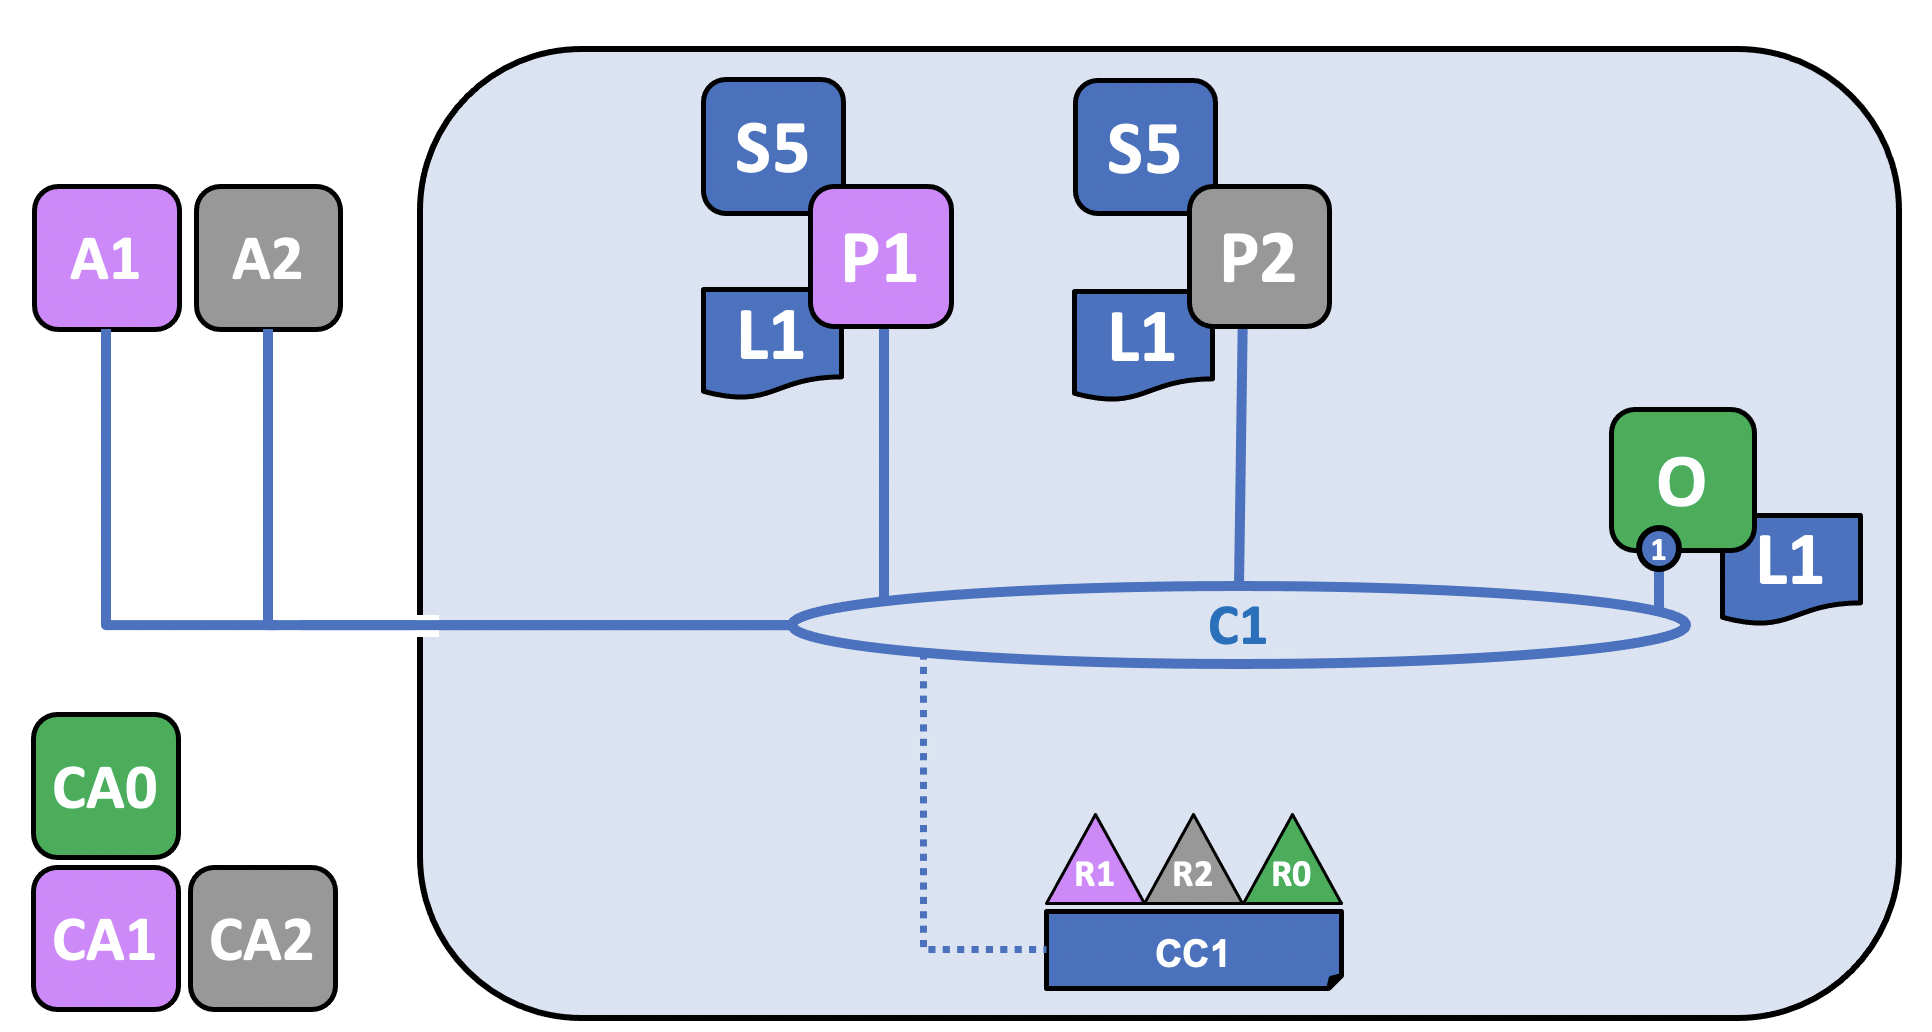
\includegraphics[width=12cm,height=12cm,keepaspectratio]{photos/network.diagram.1.png}
    \caption{A sample blockchain network between two organizations and an orderer organization, one channel and smart contracts.}
    \label{fig:hyperledger-sample-network}
\end{figure}

\bigskip
The flexibility that Hyperledger offers, in terms of setting up a private blockchain network with a modular architecture makes it the first choice for enterprise use. Pluggable CA and MSP framework, consensus policies along with the opportunity to set up complex private channel structures on the same p2p network and smart contracts in several mainstream programming languages, make it fit for a wide spectrum of scenarios. You can find several systems already in production developed using Hyperledger and a number of its sub-modules \footnote{\url{https://www.hyperledger.org/learn/blockchain-showcase}}. These are the reasons we decided to use blockchain and Hyperledger to maintain a list of shared datasets where organizations are in control without trusting a third party to maintain the system.

\section{Kubernetes}
Kubernetes or Kubernetes is an open-source tool developed by Google for orchestration, scaling, and management of containerized applications. Kubernetes operates in a cluster, which is a collection of virtual machines (VMs) overlooked by a master node. The master node is only an API server for Kubernetes admins to interact with the Kubernetes admin client instead of managing each VM separately.

\bigskip
Several cloud providers provide a managed Kubernetes cluster as Platform As A Service (PAAS) where the cloud providers are responsible for maintaining the underlying infrastructure. With implementation details like VM management and configuration of the Kubernetes cluster are kept hidden from the users and users can start using Kubernetes right out of the box. However, such a setup is not feasible for our use case. We need to set up and maintain a Kubernetes cluster ourselves so that organizations can join and leave the cluster at will and can also join nodes where data is hosted on the node itself.

\subsection{Containers}
Before going into Kubernetes, we can briefly present a background regarding container technology. Containers are the evolution of virtualization technology. Unlike virtual machines where a complete system including the physical infrastructure along with a kernel and Operating System (OS) is virtualized, containers only virtualize the OS, and off-loading the maintenance of the hardware to the host OS and sharing the kernel results in computationally very cheap virtualization technology. Containers wrap around a bare-bones OS and package all the dependencies inside an Image that can be used to spin up a replica of an application/system anywhere on any machine. And containers run completely isolated from the host system as an extra security layer so as not to affect the host machine.

\bigskip
The biggest service for container technology is Docker. Docker is available for all major operating systems and architectures. Applications can be containerized using a simple \lstinline{Dockerfile}. Docker uses the \lstinline{Dockerfile} to create an image that can then be used to spin up containers anywhere, with the same parameters, in seconds compared to minutes of virtual machine allocation and start-ups. 

\bigskip
Docker-Compose is a supplement to the bare bones docker system. Docker-compose allows packaging and running multiple containers as services; that might be dependent on each other; with a single command. Yet Another Markup Language (YAML) file can be used to describe different containers, their environment, volumes, and networks and the running of a single command spins up all the dependent services with the parameters specified. We use docker and docker-compose not only to spin up not only a test blockchain network using Hyperledger but also to allocate isolated environments for each user that logs in to use Jupyterhub.

\bigskip
Coming back to Kubernetes offerings and why we decided to use Kubernetes in our system. Kubernetes offers features such as health checks of running containers and restarts in case of node or container failures. Supports the scaling up of applications depending on the resource demand and load balancing between horizontally scaled services or scaling down in case demand goes down. Provides several, easy plug-in storage options so applications do not care about the storage infrastructure and Kubernetes can handle that whether a Cloud (Azure, AWS, or GCP) storage solution is used or a node-local one or even a network shared file system.

\bigskip
Because of the auto-scaling and optimized utilization of the resources, Kubernetes as a tool is very useful and interesting for data scientists, who frequently need to run resource-heavy simulations or analytics on often gigantic data sets. However Kubernetes has a steep learning curve and in practicality serves more use cases from a software engineer's perspective than a data scientist, even though it can be an extremely useful tool for running compute-heavy workloads. 

\bigskip
The first reason we incorporate Kubernetes into our system is the obvious benefit Kubernetes presents when running compute-heavy workloads. Also, we want to allow organizations to contribute the compute resources in addition to sharing datasets. Secondly, as discussed earlier Kubernetes offers a plug-n-play solution for using data from several sources and storage systems. We intend to leverage this feature to support a wide number of storage systems, allowing organizations flexibility to use any storage system and not causing hindrance for organizations to participate in our system. In the proof of concept we are only using Azure but because of Kubernetes wide storage support can be easily extended. Next up we intend to make use of JupyterHub, JupyterFlow, and Argo Workflow for giving users an environment to write code, construct workflows and trigger them instead of developing the environment ourselves and hence the choice to use Kubernetes. And as discussed in future work can help give weightage to the computed results, to the organizations contributing more resources towards computation as well as datasets, and then incentivize when those results are utilized or even sell their stake in the results.

\subsection{Jupyterhub}
Project Jupyter started as a simple interface providing a Jupyter notebook that provides runnable modules within itself and thus supports interactive programming. And in addition to the interactive programming support, Jupyter also provides support for running kernel commands directly from the notebook. It is one of the most widely used Integrated Development Environment (IDE) for Python and data science. Jupyter is a set of open-sourced software and standards for interactive programming across several languages but is found most used in Python settings. The notebook is still the most basic block of a Jupyter environment but it has developed into a much more diverse set of tools. We will take a look a JupyterHub in this section.

\bigskip
JupyterHub is an enterprise solution for big companies and research labs to host multi-user Jupyter environments on a server. It runs on a central server or a Kubernetes cluster and can spawn multiple instances of single-user notebook servers and hence providing each user with an isolated environment (to avoid conflicting processes and security of the underlying infrastructure). JupyterHub is designed to be containerized and Kubernetes friendly and thus can scale up and down depending on the number of users. It provides a pluggable authentication service to support several identity providers. Currently, it supports Privileged Access Management (PAM), Lightweight Directory Access Protocol (LDAP), and OAuthenticator out of the box and supports custom Authenticator Interface implementation implemented following OAuth standards. One of the projects alongside this thesis is to develop a Distributed Identity using blockchain and a custom Authenticator for JupyterHub. The integration with DID framework and using the custom authenticator falls out of the scope of this project. These all features combined make it a perfect tool for a consortium of organizations to serve users with a single-point solution for data analytics. 

\bigskip
Jupyter has grown from a single notebook to an array of tools and JupyterLab is the next generation of the Jupyter interface. JupyterLab is a completely new extensible interface for Jupyter. Unlike the classic notebook interface, JupyterLab is designed from the ground up to be a modular solution and a complete integrated environment with powerful tools like a file explorer, multiple programming language kernels and terminals, and editors with embedded debuggers. In addition to all this, JupyterLab allows the use and motivates the development of community-driven third-party extensions. We turn on the JupyterLab interface on JupyterHub and develop a custom extension to explore the datasets. All these features of JupyterHub and JupyterLab make it the ideal tool for the development of a workflow management system aimed at allowing organizations to collaborate.

\subsection{Argo Workflow}
Argo workflow is an open-source tool or Custom Resource Definition for Kubernetes that provides the ability to define complex workflows and can trigger them on Kubernetes. In Argo we can specify each job in the workflow as a collection of Docker images, volumes and environment variables and Argo can spin up the respective pods. Argo also provided the functionality to specify dependencies among workflow jobs as Directed A-cyclic Graphs (DAG) and takes care of triggering jobs in the order of our workflow, triggering parallel jobs together and waiting for dependant jobs to finish before triggering the next one.

\bigskip
After installing Argo Workflow, we can start writing YAML files for workflows that can be consumed by Argo to trigger pods on Kubernetes. Argo also exposes a web User Interface (UI) for users to see the workflows triggered, monitor them for errors and check logs, etc. Another useful feature of Argo is exit handlers, which enable the user to specify exit strategies in case of success or failure both, to clean up the resources that Argo was consuming. We have not managed to utilize this feature in this thesis but we discuss how it can be useful in future work \ref{ch:conclusion}.

\subsection{JupyterFlow}
As discussed earlier, the auto-scaling nature of Kubernetes and now tools like JupyterHub that run natively on Kubernetes, make it the ideal solution to run computationally heavy machine learning or statistical workflows on. However Kubernetes has a relatively steep learning curve and as data scientists, our energies need to be focused on data rather than configuring and working towards running our workflows on Kubernetes. Before we can run our workflows on Kubernetes we need to containerize our code along with any environment configurations. To allow data scientists to use Kubernetes to run their workflows without tinkering too much with Kubernetes we need an abstract tool that can handle Kubernetes configuration and configuration details on its own and allow us as a user to just run workflows. JupyterFlow \cite{jupyterflow} is this tool, distributed as a Package Installer for Python (PIP) package.

\bigskip
JupyterFlow is a tool that is logically built on top of JupyterHub on K8s and Argo Workflows. As discussed in the previous subsection Argo allows writing YAML workflows as custom Kubernetes objects and takes responsibility to trigger the respective pods in the order that workflow requires. JupyterFlow uses Argo and Kubernetes API under the hood and makes it even simple for us as data scientists to focus on data and not take on a role of a software engineer. It takes the image and environment that JupyterHub uses to spin up the Jupyter instance for the user and a very simplified YAML file and constructs an Argo workflow and then triggers it on the Kubernetes cluster.

\bigskip
The only limitation for JupyterFlow is that it only works on JupyterHub on Kubernetes. Since we already have chosen to use JupyterHub on Kubernetes as a platform for users to work on, JupyterFlow fits perfectly into our scenario and we can extend it to use custom volumes on each job while still maintaining the simplicity, that JupyterFlow brings.

\bigskip
JupyterFlow removes the overhead of containerizing the code and writing insanely complex Argo YAML files to run the complex workflows on a Kubernetes cluster. Since JupyterHub on Kubernetes can spawn up a separate single-user Jupyter instance for every user that logs in by using a pre-built docker image with all the dependencies installed and environment setup. As JupyterFlow runs on top of JupyterHub on K8s, it can use the Kubernetes API to get the image used for setting up the environment and fetch the volume details for the user's home directory. JupyterFlow can use these two details to containerize the environment without users' intervention. To pass the code the user has been working with inside the Jupyter server, it utilizes the shared storage solutions that JupyterHub on Kubernetes offers natively. Since each user gets their shared access storage so the code and files the user works with are already accessible to Kubernetes we only need to make it available to the workflow that Kubernetes is gonna run. After these details have been fetched, JupyterFlow uses a template of Argo workflows to compile the Argo workflow YAML file from the simple YAML file provided by the user. In this way, JupyterFlow removes the overhead of learning Kubernetes and writing complex workflow YAML files. It can take a simple YAML file \ref{lst:basic-jflow} and takes care of containerizing, creating Argo workflows from it, and triggering it on Kubernetes.

\section{Storage Solutions}
The last piece of the puzzle for our proof of concept is the storage solutions we can support to consume. Most organizations are moving their on-premise infrastructure to the cloud or a hybrid model. And cloud storage gives them the flexibility to store enormous amounts of data without the hassle of maintaining the infrastructure. Cloud Providers offload the responsibility and make the data highly available, scalable, and secure through Role-Based Access Control (RBAC). 

\bigskip
Kubernetes can support mounting volumes for containers from several storage sources. In this thesis, we develop the system to support Azure Fileshare and Storage on Kubernetes Nodes as the two available storage solutions. We opt for Microsoft's Azure platform owning to the huge presence in the Nordics and the great resources available. We make use of Azure Fileshare which organizations can use to store their data and when needed we can mount the Fileshare on the Kubernetes Cluster, may be residing in the same data center and using the data for analytics without giving up the ownership of the data itself to the consuming user. 

To summarize we have discussed in this section the technologies we have chosen to develop our proof of concept and why we have chosen the technologies. And a brief overview of what is the responsibility of each component. \ref{fig:component-jobs} highlights a visual representation of all the components involved in the system and what function each component serves in our architecture.

\begin{figure}
    \centering
    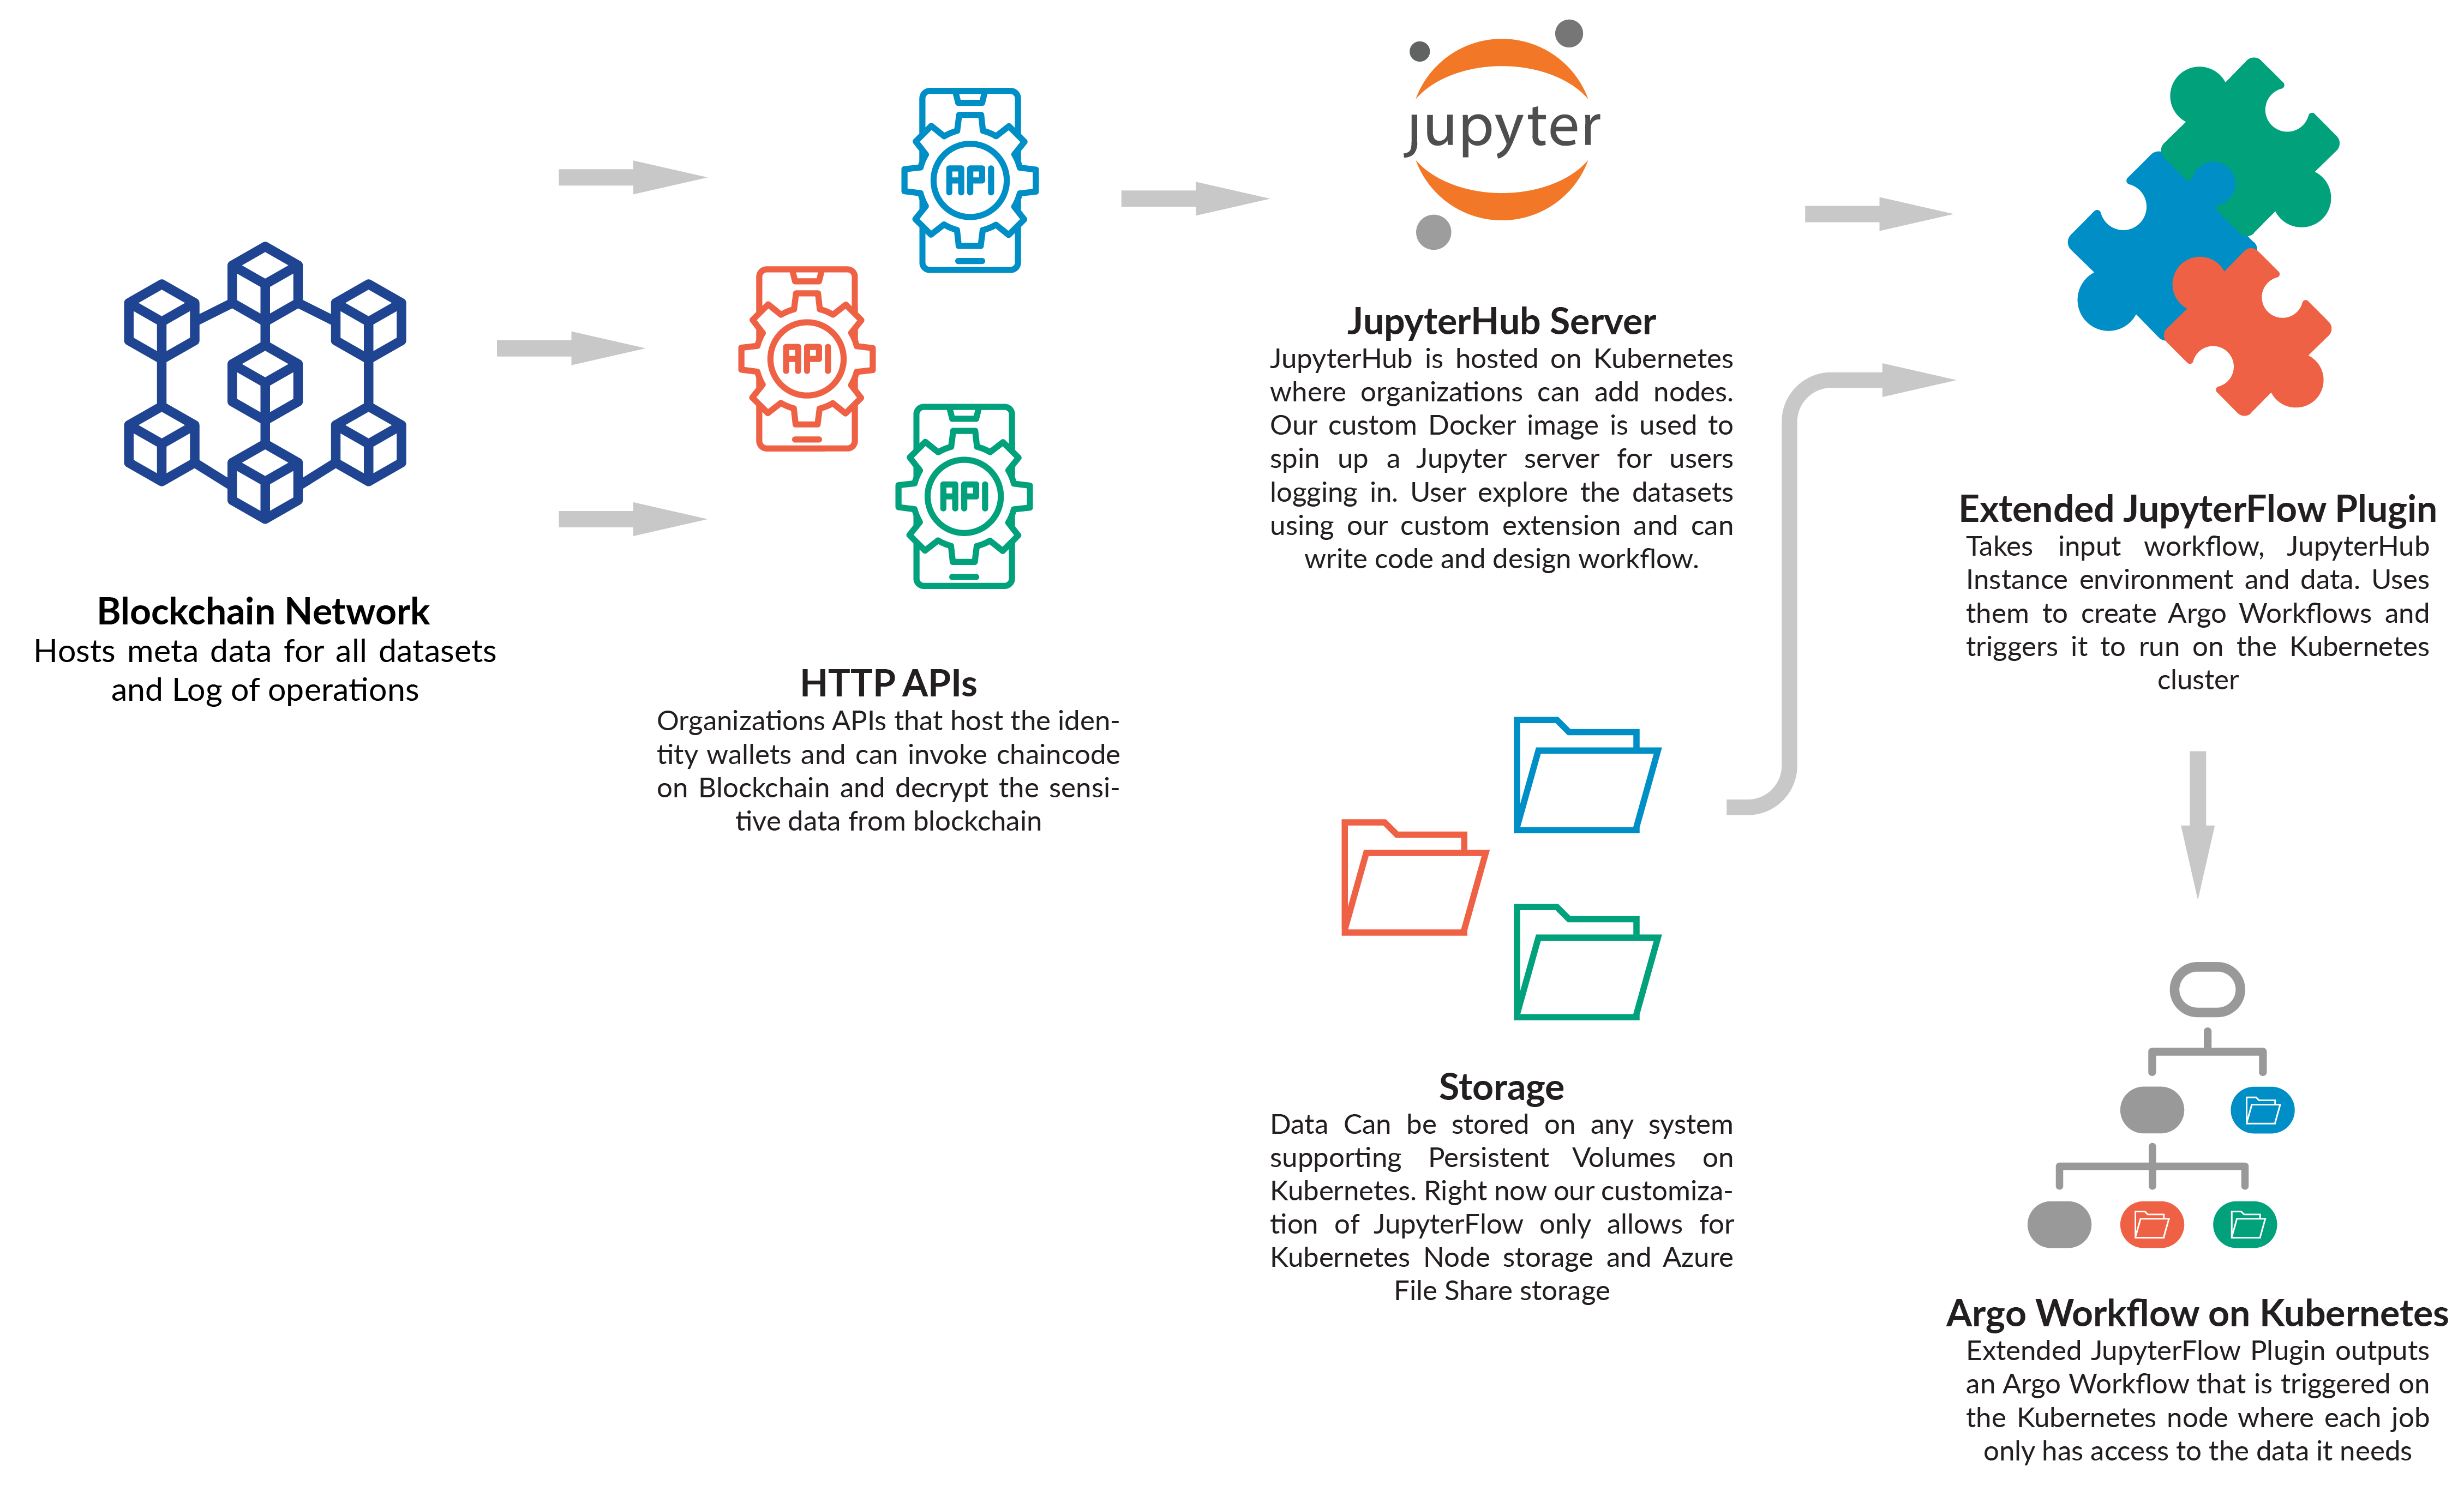
\includegraphics[width=14cm,keepaspectratio]{photos/overview.png}
    \caption{The tools and technologies discussed in background section and how they all integrate and work together in the proposed system.}
    \label{fig:component-jobs}
\end{figure}